%!TEX root = ../document.tex
\chapter{DNS-Spoofing}
In diesem Angriff wird auf das Domain Name System (DNS) eines Rechners zugegriffen, um die Zuordnung zwischen Domainnamen und zugehöriger IP-Adresse zu fälschen. Damit kann der Datenverkehr unbemerkt auf einen anderen Computer gelenkt werden, um z.B. Phishing- oder DoS-Angriffe durchzuführen.

\section{Erklärung}
\begin{figure}[H]
	\centering
	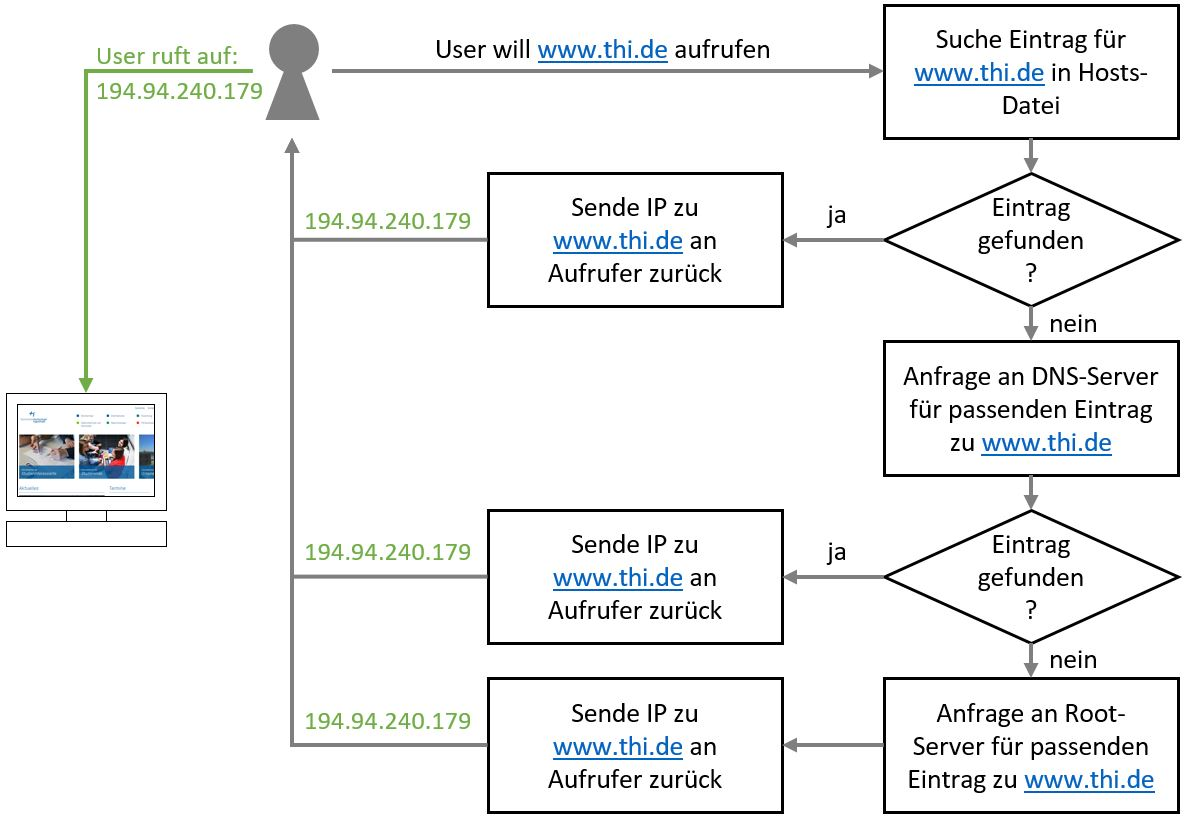
\includegraphics[width=\textwidth]{images/dns_spoofing/normal_dns_lookup.jpg}
	\caption{Vorgehen eines DNS-Lookups}
	\label{fig:normal_dns_lookup}
\end{figure}

Die Adressierung und der anschließende Verbindungsaufbau zu einem Server erfolgt über eine eindeutige IP-Adresse. Da IP-Adressen im Allgemeinen sehr schlecht lesbar sind (z.B. 194.94.240.179) wurde das Domain Name System (DNS) eingeführt. Dieses ordnet jeder IP-Adresse einen für den Menschen verständlichen Namen (Domain Name) hinzu (z.B. www.thi.de). DNS ähnelt somit der Funktionsweise eines Telefonbuchs.

Abbildung \ref{fig:normal_dns_lookup} zeigt, wie die Suche nach der IP-Adresse normalerweise erfolgt. Zuerst wird in einem lokalen Zwischenspeicher (Cache) nach einer IP-Adresse gesucht, die zum Domain-Name \enquote{www.thi.de} gehört. Ist im lokalen Cache kein Eintrag enthalten, wird in einem DNS-Server weiter gesucht. Ein DNS-Server steht vielen Hosts zur Verfügung und hält eine große Anzahl von IPs bzw. Domain-Namen vorrätig. Ist auch hier kein entsprechender Eintrag vorhanden, wird die Anfrage an den Root-Server weitergeleitet. Der Root-Server ist ein allwissender DNS-Server, der einen Verweis auf einen weiteren DNS-Server geben kann, der die notwendigen Informationen enthält. Es gibt über die Welt verteilt 13 Root-Server.

Beim DNS-Spoofing versucht der Angreifer nun, dem Opfer einen gefälschten DNS-Eintrag unterzuschieben:
\begin{lstlisting}[caption=Echtes vs. gefälschtes DNS]{Name}
Korrekter DNS-Eintrag:   194.94.240.179  - www.thi.de
Gefälschter DNS-Eintrag: 123.123.123.123 - www.thi.de
\end{lstlisting}

Dabei nutzt der Angreifer die Antwortzeit zwischen DNS-Server und Opfer aus. Der Angreifer verfolgt den Netzwerkverkehr des Angegriffenen und sendet einen gefälschten DNS-Eintrag los, sobald das Opfer einen Eintrag suchen muss. Der PC des Opfers erhält den gefälschten DNS-Eintrag zu \enquote{www.thi.de} mit der IP-Adresse 123.123.123.123 des Angreifers, speichert diese gutgläubig im lokalen Cache ab und öffnet die Verbindung zum Server des Angreifers. Selbst wenn im Anschluss noch die richtige IP-Adresse durch den offiziellen DNS-Server geliefert wird, wird diese in der aktuellen Session nicht mehr berücksichtigt. Abbildung \ref{fig:poisoned_dns_lookup} verdeutlicht das Vorgehen beim DNS-Spoofing.

Will das Opfer nun mithilfe des Domain Name \enquote{www.thi.de} auf die Homepage der Technischen Hochschule zugreifen, landet es stattdessen auf dem Server mit der IP \enquote{123.123.123.123} des Angreifers. Dieser Angriff kann z.B. bei Banken-Homepages sehr gefährlich sein. Wenn der Angreifer die Original-Homepage entsprechend detailliert nachgebaut hat, bemerkt das Opfer u.U. gar nicht, dass es auf einer gefälschten Seite gelandet ist und teilt dem Angreifer unwissentlich alle seine Login-Daten für das Onlinebanking mit.

\begin{figure}[H]
	\centering
	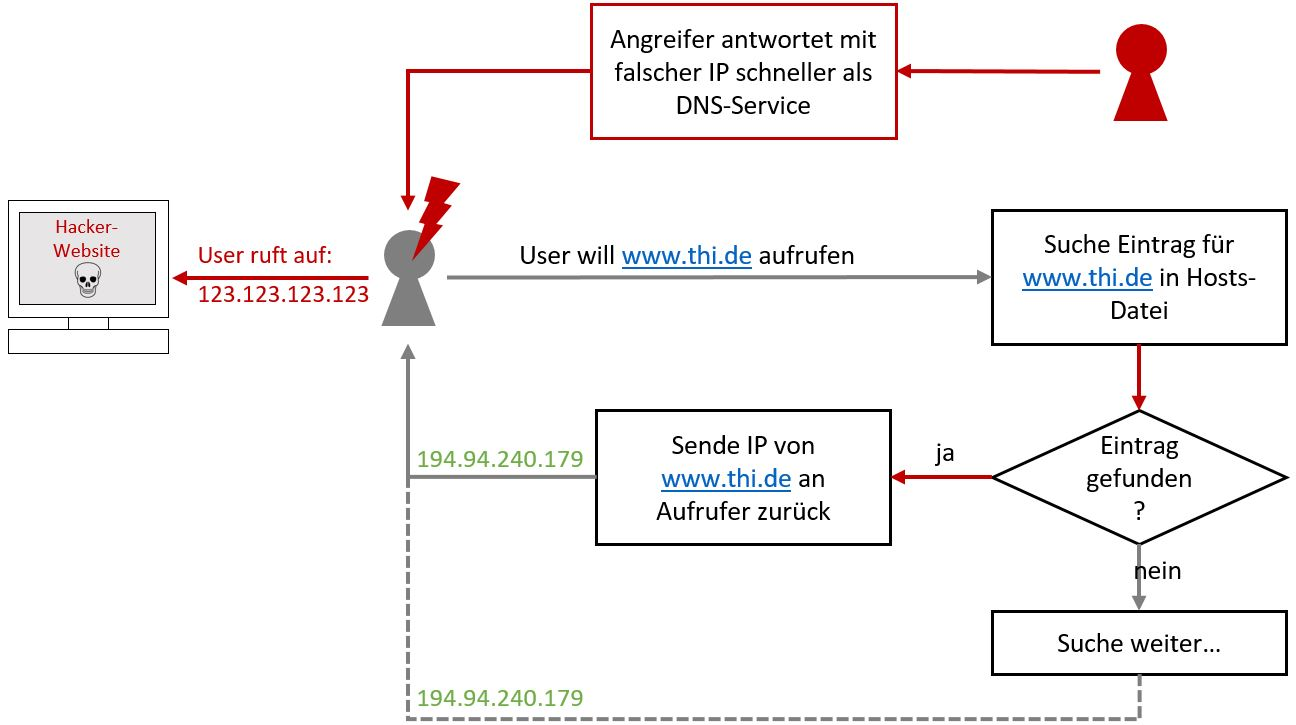
\includegraphics[width=\textwidth]{images/dns_spoofing/poisoned_dns_lookup.jpg}
	\caption{Vorgehen beim DNS-Spoofing}
	\label{fig:poisoned_dns_lookup}
\end{figure}

\section{Vorbereitung}
Für dieses Szenario gibt es kein Tutorial in der Security Workbench. Da es beim DNS-Spoofing vor allem auf die Geschwindigkeit beim Senden der Antwortnachricht - also des Angriffes - ankommt, ist dieses Tutorial nicht ohne größere Aufwände implementierbar. Der Angreifer muss mittels (\ref{chapter_arp_spoofing}: ARP-Spoofing) den Netzwerkverkehr auslesen, die Transaktions-ID (siehe nachfolgender Abschnitt) ermitteln und noch vor der aufgerufenen, legitimen IP-Adresse eine Antwort an den Client senden. 

\section{Ablauf}
Ein Client (z.B. Windows-Rechner) möchte die Internetseite der Technischen Hochschule Ingolstadt (www.thi.de) aufrufen. Dazu stellt dieser einen DNS-Request an seinen lokalen DNS-Server.
Wenn dieser lokale DNS-Server in seinem Cache keinen Eintrag findet, frägt er iterativ alle Namensserver nach ihren Einträgen ab, um zum Schluss die IP-Adresse von www.thi.de zu erhalten.

Da bei jeder DNS-Anfrage eine zufällig generierte Transaktions-ID mitgeschickt wird, und eine DNS-Antwort nur akzeptiert wird, wenn diese mit der Anfrage übereinstimmt, muss der Angreifer diese ermitteln, was sich in einem lokalen Netzwerk mit einem Sniffer sehr einfach realisieren lässt. Alternativ kann auch die Transaktions-ID erraten werden, wofür für die 16-Bit lange Transaktions-ID im Durchschnitt 32.768 Versuche notwendig sind.

\section{Gegenmaßnahmen}

Durch \emph{DNSSEC} kann die Authentizität einer DNS-Antwort verifiziert und somit DNS-Cache-Poisoning vorgebeugt werden. Durch eine asymmetrische Signatur kann der Absender der DNS-Antwort, also der DNS-Server, seine Antworten signieren, indem er mit dem nur ihm zugänglichen privaten Schlüssel den Record unterschreibt. Die Client-Seite kann anschließend im Gegenzug die Antwort mit dem öffentlichen Schlüssel des DNS-Servers überprüfen und somit verifizieren, ob die Antwort auch vom richtigen Server war.
